\begin{figure}[htbp]
\section*{ BRD4}
\centering
\begin{subfigure}[b]{0.95\textwidth}
\centering
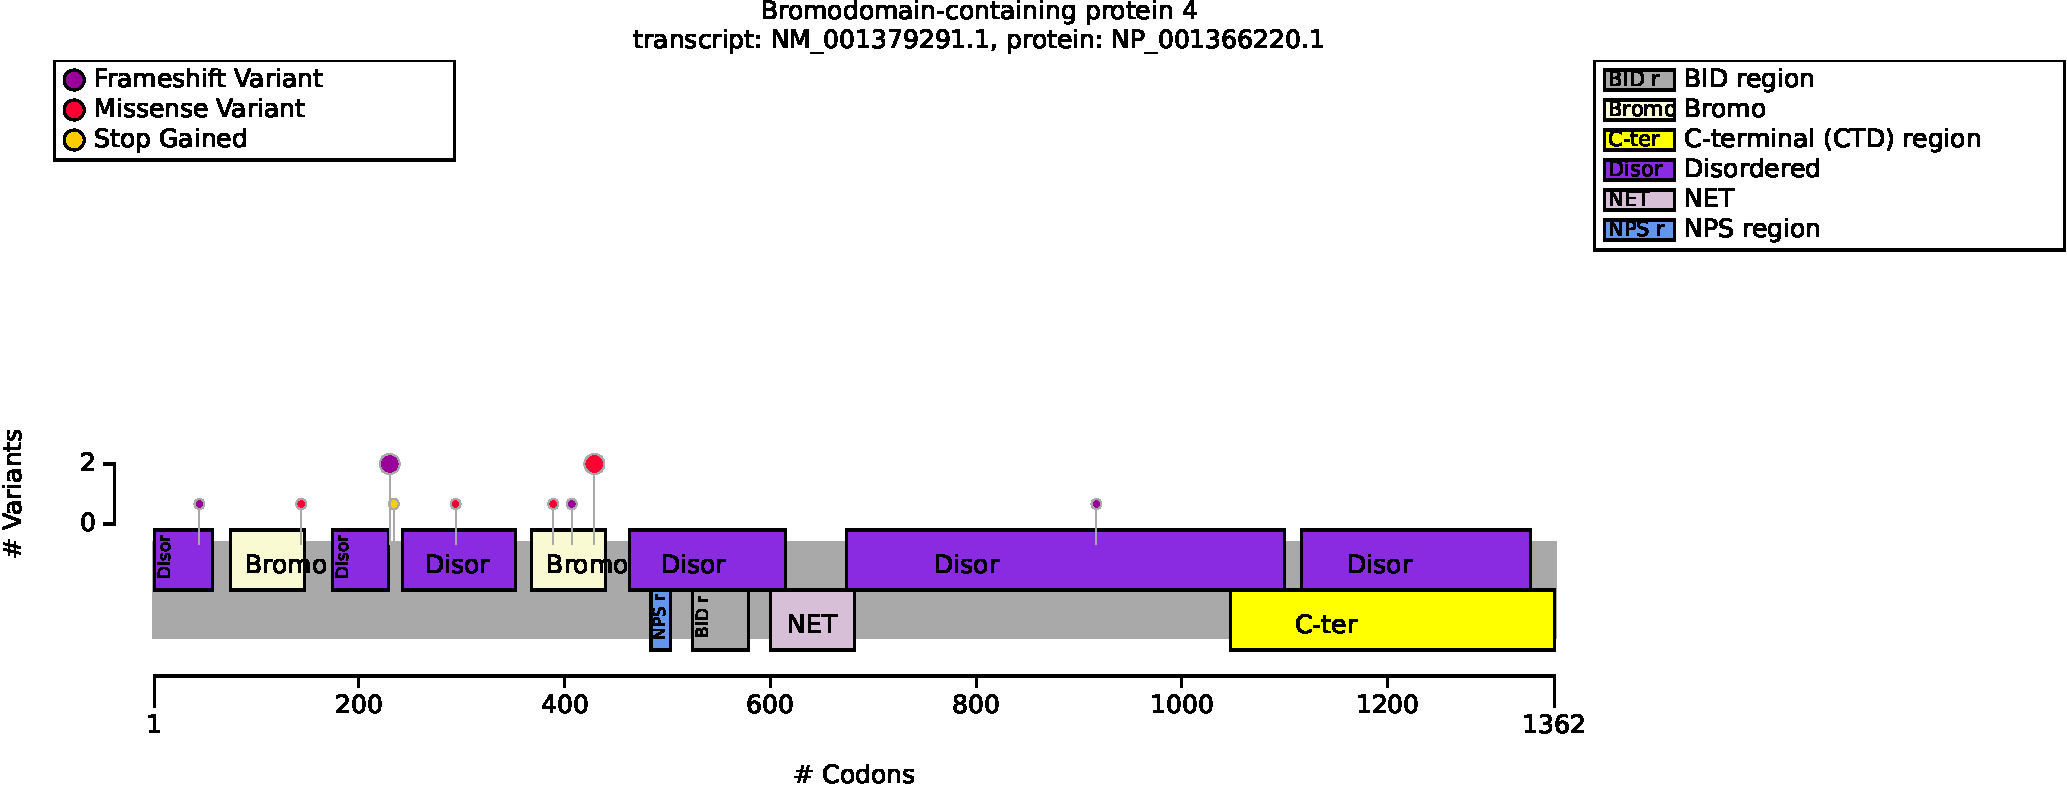
\includegraphics[width=\textwidth]{ img/BRD4_protein_diagram.pdf} 
\captionsetup{justification=raggedright,singlelinecheck=false}
\caption{Distribution of variants in BRD4}
\end{subfigure}

\vspace{2em}

\begin{subfigure}[b]{0.95\textwidth}
\centering
\resizebox{\textwidth}{!}{
\begin{tabular}{llllrr}
\toprule
HPO term & NIPBL & BRD4 & p-value & adj. p-value\\
\midrule
Intrauterine growth retardation [HP:0001511] & 37/45 (82\%) & 2/9 (22\%) & $9.45\times 10^{-4}$ & 0.032\\
\bottomrule
\end{tabular}
}
\captionsetup{justification=raggedright,singlelinecheck=false}
\caption{         Fisher Exact Test performed to compare HPO annotation frequency with respect to NIPBL and BRD4. Total of
        34 tests were performed. }
\end{subfigure}
\vspace{2em}
\begin{subfigure}[b]{0.95\textwidth}
\centering
\resizebox{\textwidth}{!}{
\begin{tabular}{llllrr}
\toprule
Genotype (A) & Genotype (B) & total tests performed & significant results\\
\midrule
ablation & other & 27 & 0\\
\bottomrule
\end{tabular}
}
\captionsetup{justification=raggedright,singlelinecheck=false}
\caption{Fisher Exact Test performed to compare HPO annotation frequency with respect to genotypes.}
\end{subfigure}

\vspace{2em}

\caption{The cohort comprised 18 individuals (8 females, 10 males). A total of 40 HPO terms were used to annotate the cohort. Disease diagnosis: Cornelia de Lange syndrome 6 (OMIM:620568). 
We compared phenotypic features of Cornelia de Lange syndrome 6 (BRD4) with those of Cornelia de Lange syndrome 1 (NIPBL).
Intrauterine growth retardation was found to be significantly more common in Cornelia de Lange syndrome 1.
A total of 10 unique variant alleles were found in \textit{BRD4} (transcript: \texttt{NM\_001379291.1}, protein id: \texttt{NP\_001366220.1}).}
\end{figure}
